\documentclass{article}

\usepackage[left=0.7in,
            right=0.7in,
            top=0.5in,
            bottom=0.7in]{geometry}
\usepackage{graphicx}
\usepackage{amsmath}
\usepackage{caption}
\usepackage{amssymb}

\newcommand{\F}{\mathscr{F}}
\newcommand{\G}{\mathscr{G}}
\newcommand{\N}{\mathbb{N}}
\newcommand{\R}{\mathbb{R}}
\newcommand{\K}{\mathbb{K}}
\newcommand{\Q}{\mathbb{Q}}
\newcommand{\Z}{\mathbb{Z}}
\newcommand{\C}{\mathbb{C}}

\DeclareMathOperator{\E}{\mathbb{E}}
\DeclareMathOperator{\Var}{Var}

\begin{document}

\section{Course content}
\begin{itemize}
    \item supervised, unpservised, reinforcement learning. classification vs clustering, Example of supervised learning and others
    \item data space with examples, example of datasets, labels, data vs task vs loss, example of common losses
    \item test set vs validation set, model complexity, params vs hyperparams,
    overfitting, underfitting, example of overfitting, example of underfitting, , 
    vbias/variance tradeoff and regularizations (lp norms, lasso ridge net)
    \item ripasso probabilita, causality vs correlation, example of causality, example of correlation, probabilita condizionata, probabilita a posteriori, probabilita a priori, joint distribution, bayes th, i.i.d
    \item gradient descent (weights and learning rate)
    \item unsupervised learnign (manifold, desnity estimation, clustering, dimensionality reduction, flat clustering (partition and density based), fuzzy clustering, hierichical clustering)
\end{itemize}

\section{What is Machine Learning}
Artificial Intelligence is the overall umbrella term for the field of developing intelligent computer systems. Machine learning is a subfield of AI that focuses on developing algorithms that can learn from data.\\
In traditional computer science, algorithms are designed to follow a set of rules or logical steps to perform a specific task.
In contrast, machine learning algorithms are designed to optimize their performance based on a given objective or metric by adjusting their parameters.
Therefore, machine learning focuses more on optimization, while traditional computer science focuses more on logical problem solving and efficient algorithm design.\\
\noindent Machine learning is growing rapidly due to several factors:
\begin{itemize}
    \item Increasing availability of data: With the proliferation of digital devices and the internet, vast amounts of data are being generated every day. This data provides an opportunity for machine learning algorithms to learn from it and improve their performance.
    \item Advancements in computing power: Machine learning algorithms require a lot of computational resources, and recent advances in computing power have made it possible to train larger and more complex models than ever before.
    \item Improved algorithms and techniques: Machine learning research has made significant progress in developing new algorithms and techniques that are more accurate, efficient, and scalable than earlier methods.
    \item Business opportunities: Machine learning has the potential to unlock new business opportunities and create efficiencies in existing industries. Companies are increasingly adopting machine learning to automate tasks, optimize processes, and make better decisions.
    \item Availability of open-source tools and frameworks: The availability of open-source machine learning tools and frameworks such as TensorFlow, PyTorch, and scikit-learn has made it easier for developers to experiment with machine learning and build custom models.
    \item Interdisciplinary collaborations: Machine learning is a highly interdisciplinary field that draws on expertise from computer science, mathematics, statistics, and other domains. Collaboration between experts from different fields is driving innovation and expanding the boundaries of what's possible with machine learning.
\end{itemize}
These factors, among others, are contributing to the rapid growth of machine learning and its increasing adoption in various industries and domains.

\noindent Here are some applications of machine learning:
\begin{itemize}
    \item \textbf{Chemistry}: Machine learning is used to predict the properties of molecules, design new drugs, and improve the efficiency of chemical processes. It is also used in materials science to predict the behavior of materials and design new materials with specific properties.
    
    \item \textbf{Medicine}: Machine learning is used for medical diagnosis, personalized treatment plans, drug discovery, and clinical decision making. It is also used in healthcare management to optimize resource allocation and reduce costs.

    \item \textbf{Mathematics}: Machine learning is used to solve complex mathematical problems, such as optimization and numerical analysis. It is also used in data analysis and pattern recognition in various branches of mathematics, such as algebra, topology, and geometry.
    
    \item \textbf{Self-driving cars}: Machine learning algorithms are used to process sensor data and make decisions in real-time for autonomous vehicles. This includes object detection, tracking, and recognition, as well as route planning and decision making based on environmental conditions.
    
    \item \textbf{AlphaGo (DeepMind)}: Machine learning was used to develop the AlphaGo program, which became the first computer program to defeat a human world champion at the board game Go. This was a significant achievement in the field of artificial intelligence and demonstrated the potential of machine learning in complex decision making.
    
    \item \textbf{Image processing and computer vision}: Machine learning algorithms are used to detect and recognize objects and patterns in images and videos. This includes face recognition, object detection, and image segmentation. Machine learning is also used in 3D computer vision, such as reconstructing 3D models from multiple 2D images.
    
    \item \textbf{Natural language processing (NLP)}: Machine learning is used to analyze and generate human language. This includes tasks such as language translation, sentiment analysis, and speech recognition. NLP is used in various applications, such as virtual assistants, chatbots, and language learning tools.
    
    \item \textbf{Fraud detection}: Machine learning algorithms are used to detect and prevent fraudulent activities in various domains, such as finance, e-commerce, and insurance. This includes identifying patterns of fraudulent behavior and predicting the likelihood of fraudulent activities.
    
    \item \textbf{Recommendation systems}: Machine learning is used to build recommendation systems that suggest products, services, or content to users based on their preferences and behavior. This includes collaborative filtering, content-based filtering, and hybrid approaches.
    
    \item \textbf{Predictive maintenance}: Machine learning is used to predict equipment failure and maintenance needs in various industries, such as manufacturing, transportation, and energy. This includes analyzing sensor data and other parameters to predict when maintenance is needed to prevent equipment failure and reduce downtime.
    
    \item \textbf{AlphaFold}: Machine learning was used to develop the AlphaFold program, a computer program to predict the 3D structure of a protein from its amino acid sequence.
    \begin{figure}[!h]
        \centering
        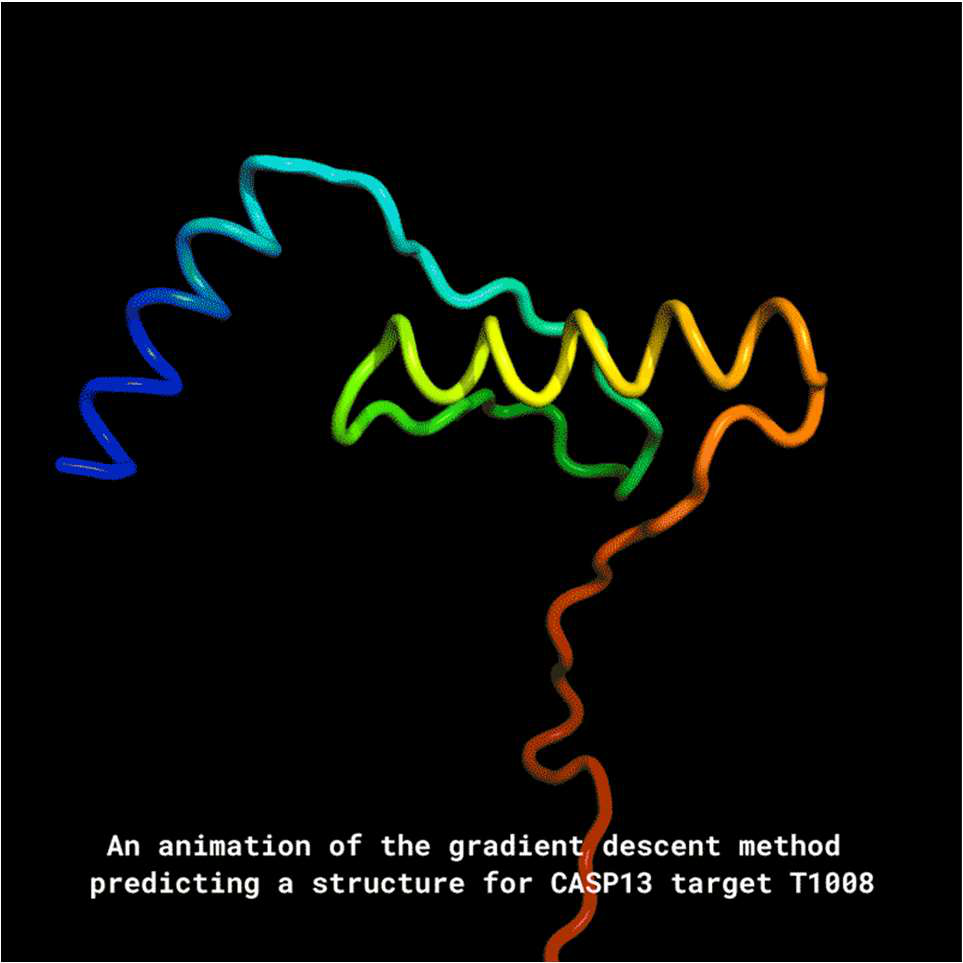
\includegraphics[width=4.5cm]{./images/p30_img183.png}
        \caption{AlphaFold}
    \end{figure}
\end{itemize}

\section{Machine Learning types}
\textbf{Supervised Learning:}
Supervised learning is a type of machine learning where the algorithm is trained on labeled data, where the correct output is provided for each input. The goal is to learn a function that maps inputs to outputs by finding patterns in the data. The algorithm can then use this function to make predictions on new, unseen data. Examples of supervised learning problems include:

\begin{itemize}
\item Classification: In classification, the goal is to predict a categorical variable based on a set of input features. For example, predicting whether an email is spam or not based on its content.
\item Regression: In regression, the goal is to predict a continuous variable based on a set of input features. For example, predicting the price of a house based on its size, location, and other features.
\end{itemize}
\textbf{Unsupervised Learning:}
Unsupervised learning is a type of machine learning where the algorithm is trained on unlabeled data, where the correct output is not provided. The goal is to find patterns or structure in the data without any prior knowledge of what the output should be. Examples of unsupervised learning problems include:

\begin{itemize}
\item Clustering: In clustering, the goal is to group similar data points together based on their features. For example, clustering customers based on their purchasing behavior to identify different market segments.
\item Dimensionality Reduction: In dimensionality reduction, the goal is to reduce the number of input features while preserving as much information as possible. For example, reducing the number of features in an image to make it easier to process.
\end{itemize}
\textbf{Reinforcement Learning:}
Reinforcement learning is a type of machine learning where the algorithm learns by interacting with an environment and receiving feedback in the form of rewards or penalties. The goal is to learn a policy that maximizes the cumulative reward over time. Examples of reinforcement learning problems include:

\begin{itemize}
\item Game Playing: In game playing, the goal is to learn a strategy that maximizes the chances of winning a game. For example, learning to play chess or Go.
\item Robotics: In robotics, the goal is to learn a policy that allows a robot to perform tasks in a dynamic environment. For example, learning to navigate a maze or pick up objects.
\end{itemize}
Overall, supervised, unsupervised, and reinforcement learning are three major categories of machine learning algorithms, each with their own characteristics and applications.\\
\textbf{Classification versus Clustering:}
\begin{itemize}
\item Classification: Classification is a type of supervised learning problem where the goal is to predict a categorical variable based on a set of input features. Examples include predicting whether an email is spam or not, or whether a patient has a particular disease based on their symptoms.
\item Clustering: Clustering is a type of unsupervised learning problem where the goal is to group similar data points together based on their features, without any prior knowledge of what the groups should be. Examples include clustering customers based on their purchasing behavior, or clustering genes based on their expression levels.
\end{itemize}
\begin{figure}[!ht]
    \centering
    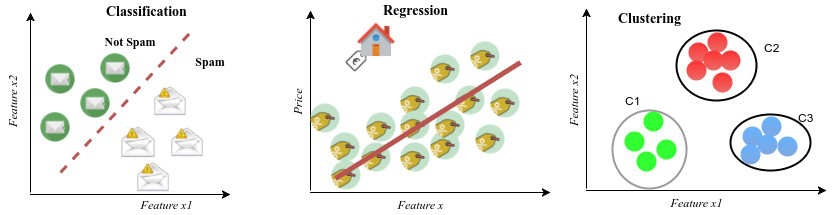
\includegraphics[width=\textwidth]{./images/p50_img275.png}
    \caption{Example of classification, regression, clustering}
\end{figure}
Classification and clustering are used for discrete data, where the input features are categorical or discrete values.\\
\section {Basic definitions}
The term \textbf{data space} refers to the set of all possible inputs that the model can receive.\\
On the other hand, the \textbf{label space} refers to the set of all possible outputs that the model can produce.\\\\
To give a concrete example, consider the CIFAR-10 dataset, which consists of 60,000 32x32 color images in 10 classes, with 6,000 images per class.
In this dataset, the data space would be the set of all possible 32x32 color images, while the label space would be the set of 10 possible classes: airplane, automobile, bird, cat, deer, dog, frog, horse, ship, and truck.
A machine learning model trained on this dataset would take an input image from the data space and produce an output label from the label space.\\\\
\begin{figure}[!ht]
    \centering
    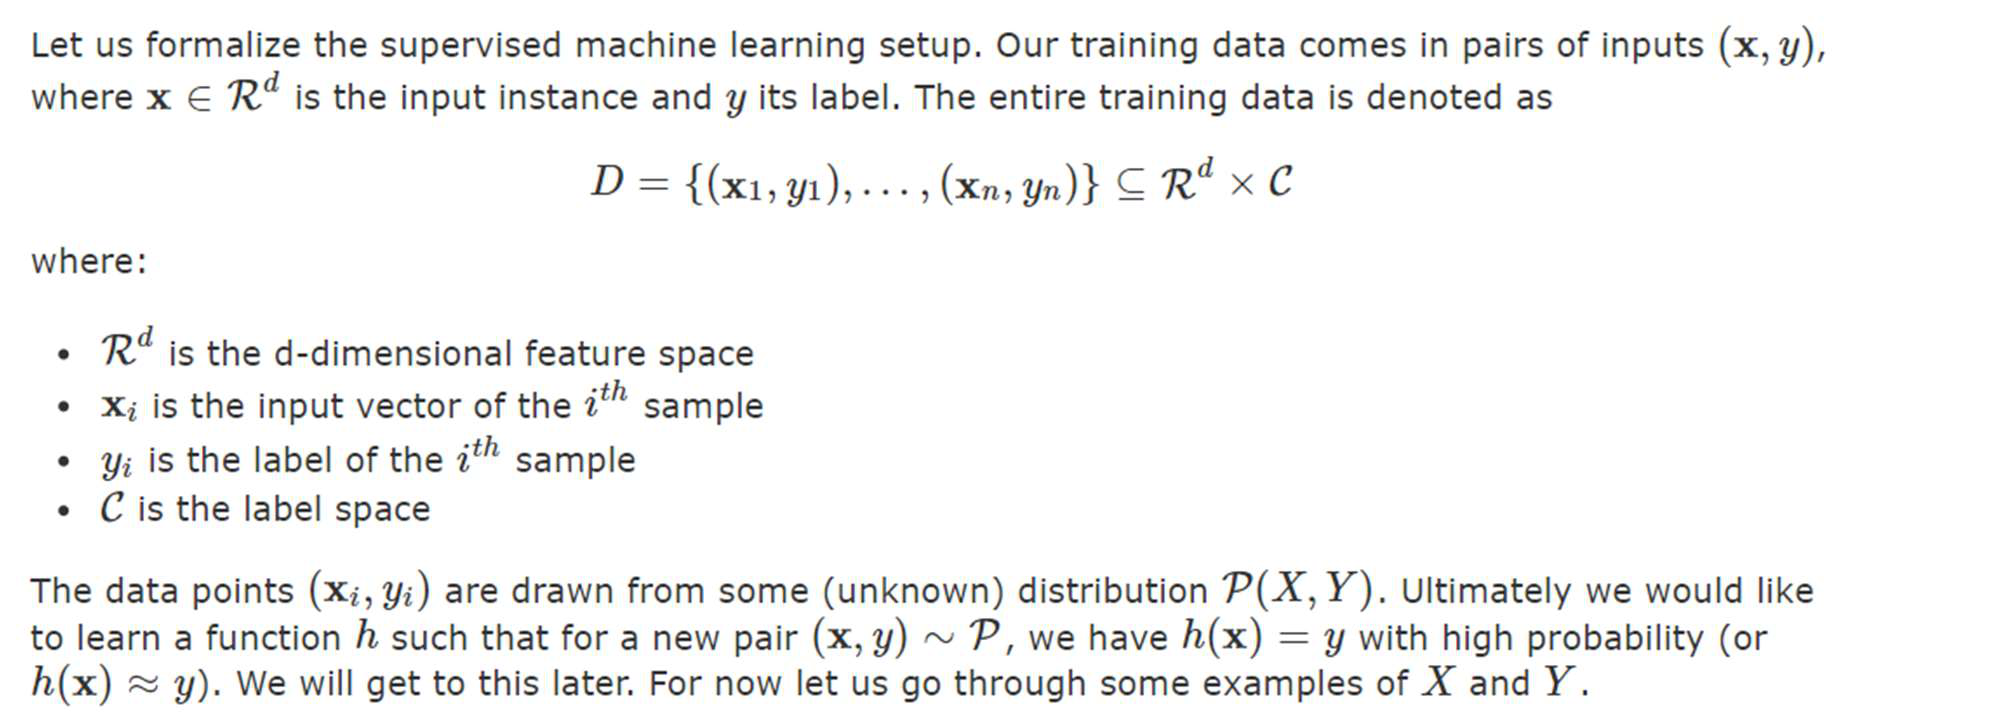
\includegraphics[width=\textwidth]{./images/p63_img322.png}
\end{figure}

\noindent The task refers to the goal of the machine learning model. For example, in an image classification problem, the task might be to correctly predict the label of an image given its input.\\
The model is a mathematical function that maps the input data to the output label.\\
The loss is a mathematical function that measures the difference between the predicted output of the model and the true output. The goal of training the model is to minimize this loss function.\\
Commonly used loss functions in machine learning include:
\begin{itemize}
    \item Mean squared error (MSE): Used for regression problems, the MSE measures the average squared difference between the predicted and true values.
    \[\frac{1}{N} \sum_{i=1}^N (y_i-\hat{y}_i)^2\]
    RMSE is the square root of MSE, which makes it easier to interpret because it is in the same units as the target variable but it is more sensitive to outliers than MSE. 
    \item Cross-entropy: Used for classification problems, cross-entropy measures the difference between the predicted and true probability distributions over the classes.
    \[\sum_i y_i \ln{p(x_i)} + (1-y_i) \ln{(1-p(x_i))}\]
    \item Binary cross-entropy: A variant of cross-entropy used for binary classification problems where there are only two possible classes.
    \[\text{FORMULA}\]
    \item Hinge loss: Used for classification problems in which the model is expected to produce a binary output, the hinge loss measures the difference between the predicted output and the true output.
    \[\text{FORMULA}\]
    \item KL divergence: Measures the difference between the predicted and true probability distributions over the classes or categories.
    \[\text{FORMULA}\]
\end{itemize}
\section{Dataset processing}
Splitting a dataset is a common practice in machine learning to evaluate the performance of a model and prevent overfitting. Typically, a dataset is split into two or three subsets: a training set, a validation set (sometimes), and a test set.\\
\begin{itemize}
    \item Training set: This subset of data is used to train the machine learning model. The model learns from the patterns in the training data and adjusts its parameters to minimize the loss function. This is the largest subset of data, typically around 70-80% of the total data, and should be representative of the underlying distribution of the data.
    \item Validation set: This subset of data is sometimes used to tune the hyperparameters of the model. Hyperparameters are settings of the model that are not learned from the data, such as the learning rate or the number of layers in a neural network. The validation set is not used for training, but instead provides a way to evaluate different choices of hyperparameters and select the best ones.
    \item Test set: This subset of data is used to evaluate the performance of the final model after it has been trained and tuned. The test set should be representative of the real-world data that the model will encounter in practice, and should not be used for training or tuning the model.
\end{itemize}
The goal is to ensure that the model is robust and generalizes well to new data.\\
\section{Model complexity and overfitting}
Model complexity refers to how flexible or expressive a machine learning model is in terms of its ability to capture patterns in the data. A simple model has a low level of complexity and may be easy to interpret, but may not capture all of the important patterns in the data.\\
A complex model, on the other hand, has a high level of complexity and may capture more of the patterns in the data, but may be harder to interpret and more prone to overfitting.\\\\
Overfitting occurs when a model is too complex and learns the noise or random variations in the training data, instead of the underlying patterns. This leads to poor generalization performance, where the model performs well on the training data but poorly on new, unseen data. An example of overfitting is a decision tree that has many levels and splits, which captures all the noise in the training data and does not generalize well to new data.\\\\
Underfitting occurs when a model is too simple and cannot capture the underlying patterns in the data, leading to poor performance on both the training and test sets. An example of underfitting is a linear regression model that tries to fit a non-linear relationship between the input and output variables, and does not capture the true pattern in the data.
\begin{figure}[!ht]
    \centering
    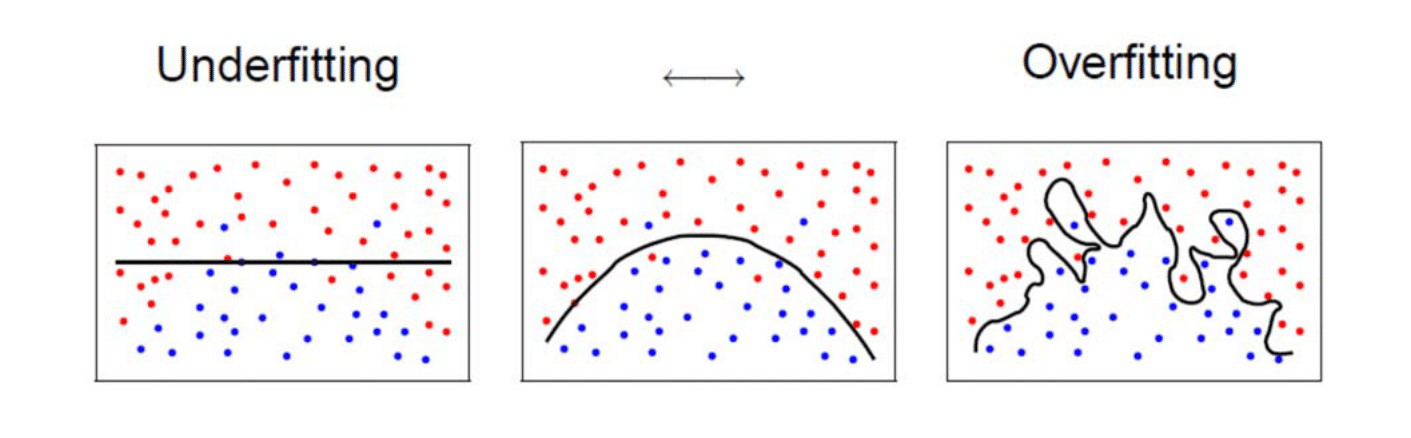
\includegraphics[width=\textwidth]{./images/p93_img447.png}
    \caption{Example of overfitting and underfitting}
\end{figure}

\[\text{TODO INSERT EXAMPLE OF LIN. REGRESS. TO A CURVE}\]
\newpage
\section{Bias-variance tradeoff}
The bias-variance tradeoff is the balance between the complexity of the model and its ability to generalize well to new data.\\
\begin{figure}[!ht]
    \centering
    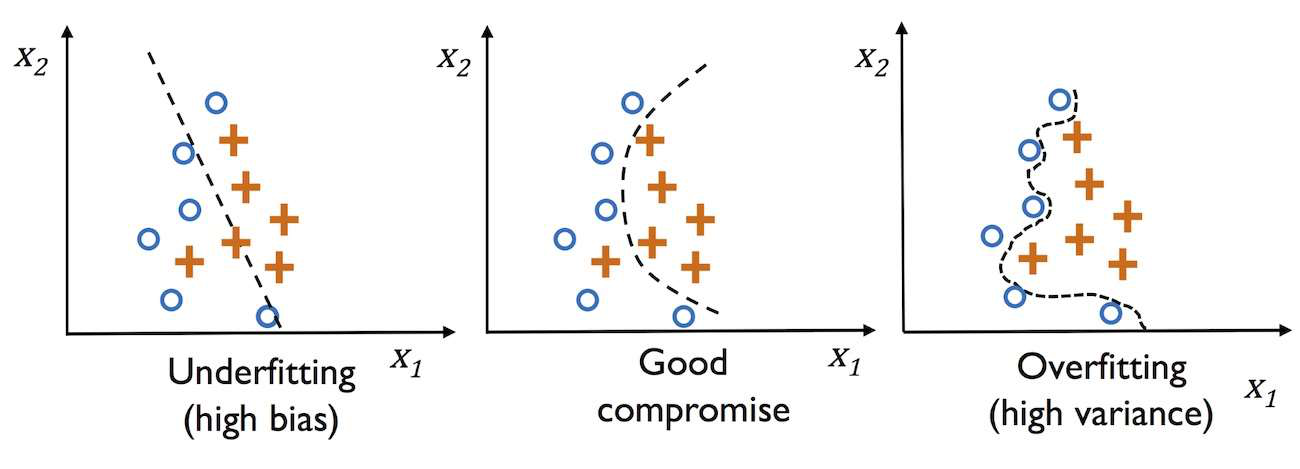
\includegraphics[width=11cm]{./images/p112_img523.png}
    \caption{Overfitting and underfitting}
\end{figure}

\noindent Bias refers to the error that is introduced by approximating a real-world problem with a simpler model, while variance refers to the error that is introduced by model sensitivity to small fluctuations in the training data.\\
A high-bias model may have poor performance on the training data but generalizes well to new data, while a high-variance model may have good performance on the training data but poor generalization performance.\\
\begin{figure}[!ht]
    \centering
    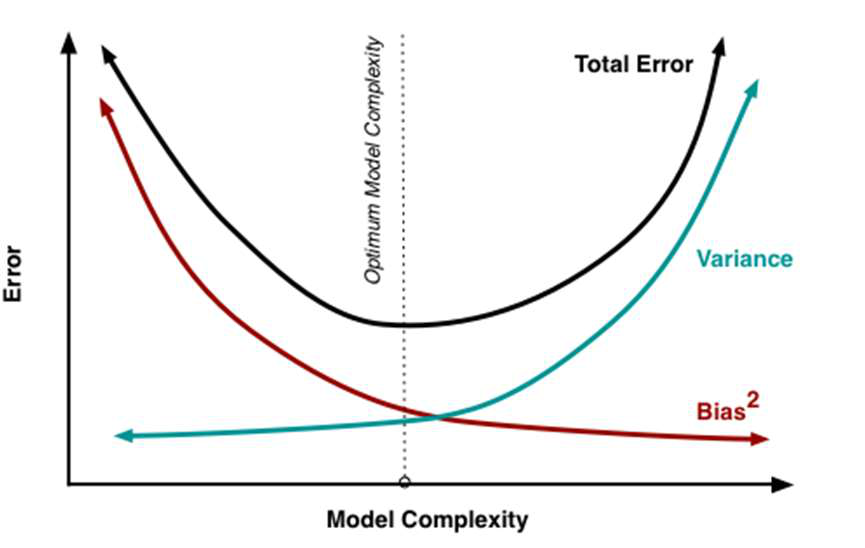
\includegraphics[width=11cm]{./images/p118_img552.png}
    \caption{Bias-variance tradeoff}
\end{figure}
\subsection{Bias-variance tradeoff in formal terms}
Consider the following model:
\[y = f(x) + \epsilon\]
where $f(x)$ is the true function that relates the input $x$ to the output $y$, and $\epsilon$ is the noise in the data.\\
$\epsilon$ is a random variable such that:
\[\E[\epsilon] = 0, \Var[\epsilon] = \sigma^2\]
When we try to model the underlying real-life problem, what this means actually is that we try to find a function $\hat{f}$ such that it is as close to the true (yet unknown to us) function f.
Function $\hat{f}$ is learned by minimizing a loss function whose goal is to bring predictions of training data as close as possible to their observed values: $y \approx \hat{f}(x)$.\\
MSE is a common loss function used in regression problems and is defined as:
\[\text{MSE} = \E[(y - \hat{f}(x))^2]\]
The bias of a model is defined as the difference of the average value of prediction (over different realizations of training data) to the true underlying function f(x) for a given unseen (test) point x.
\[\text{Bias} = \E_{\hat{f}}[\hat{f}(x) - f(x)]\]
In similar fashion, the variance of the model is defined as:
\[\text{Variance} = \E_{\hat{f}}[(\hat{f}(x) - \E_{\hat{f}}[\hat{f}(x)])^2]\]
The formula that relates the bias and variance of a model is:
\[\E_x[\E_{\hat{f}, \epsilon}[(y - \hat{f}(x))^2]] = \E_x[\text{Bias}^2 + \text{Variance} + \sigma_\epsilon^2]\]
The first expectation term is over the distribution of unseen (test) points x, while the second over the distribution of training data and random variable $\epsilon$.\\
Note: $\E_{\hat{f}, \epsilon}$ is the expectation over the model and the noise (the model and the noise depend on the training data).\\\\
The formula can be written in a more compact form:
\[\E[\E[(y - \hat{f}(x))^2]] = \E[\text{Bias}^2] + \E[\text{Variance}] + \sigma_\epsilon^2\]
or can be found in this form:
\[\text{MSE} = \text{Bias}^2 + \text{Variance} + \sigma_\epsilon^2\]
where $\sigma_\epsilon^2$ is the irreducible error, which is the error that cannot be reduced by any model.\\
The formula can be proven by using properties of expectation value. TODO\\
https://towardsdatascience.com/the-bias-variance-tradeoff-8818f41e39e9

\section{Model parameters and hyperparameters}
In machine learning, the terms "model parameters" and "hyperparameters" refer to two different types of values that are used to train a model.\\
Model parameters are the variables that are learned by the model during training, based on the input data and the desired output. These parameters are adjusted by the learning algorithm in order to minimize the difference between the predicted output of the model and the true output.\\
For example, in a linear regression model, the model parameters are the slope and intercept of the line.
Hyperparameters, on the other hand, are values that are set before training begins and are not learned by the model during training. They control aspects of the learning algorithm, such as the learning rate, the number of hidden layers in a neural network, or the type of regularization used.
\subsection{Regularization hyperparameters}
Regularization is a technique used to reduce the complexity of a model by adding a penalty term to the loss function that the model is trying to minimize. The penalty term is typically based on the magnitude of the model parameters and is intended to discourage the model from assigning too much weight to any one feature or input. Regularization helps to prevent overfitting, which occurs when the model is overly complex and fits the training data too closely, resulting in poor performance on new, unseen data.\\
There are several types of regularization techniques, including L1 regularization (also known as Lasso), L2 regularization (also known as Ridge regression), and dropout regularization. L1 regularization adds a penalty term proportional to the absolute value of the model parameters, while L2 regularization adds a penalty term proportional to the square of the model parameters. Dropout regularization randomly drops out some of the nodes in a neural network during training, forcing the remaining nodes to learn more robust features.\\
By adding regularization to a model, it is possible to achieve better generalization performance on new data, even if the model is less accurate on the training data. This is because the model is less likely to overfit and will be better able to generalize to new, unseen data.\\
\noindent For example, in linear regression models, the lasso regularization term is added to the loss function as:
\[\text{Lasso loss} = \frac{1}{n} \sum_{i=1}^n (y_i - \hat{f}(x_i))^2 + \lambda \sum_{j=1}^p |\omega_j|\]
that can be written in this form:
\[\text{Lasso loss} = \frac{1}{2n} ||y - X\omega||_2^2 + \lambda ||\omega||_1\]
where $\lambda$ is the regularization hyperparameter.\\\\
The difference between Lasso and Ridge regularization is the type of penalty term they use to prevent overfitting.
Lasso performs feature selection by setting some regression coefficients to zero, while Ridge performs coefficient shrinkage by reducing the magnitude of all the regression coefficients.\\
Limitations of Ridge and Lasso Regressions:
\begin{itemize}
    \item Ridge regression does not help in feature selection.
    \item Ridge regression use to shrink the coefficients, but never sets their values as absolute zero.\\
    The model will retain all the features and will remain complex, which may lead to poor model performance.
    \item When we apply Lasso regression to a model which has highly correlated variables, then it will retain only a few variables and sets other variables to be zero. That will lead to some loss of information as well as lower
    accuracy of the model.
\end{itemize}
We can combine Lasso and Ridge regularization techniques to obtain a hybrid regularization method that balances the strengths of both methods.
This hybrid regularization method is known as Elastic Net.\\
Elastic Net regularization is particularly useful for datasets with a large number of features and multicollinearity between predictors, as it can handle highly correlated predictors by selecting one predictor from a group of highly correlated predictors while shrinking the coefficients of the others towards zero.

\section{Supervised learning models}
\subsection{Linear regression}
Linear regression is a statistical method used to model the relationship between a dependent variable and one or more independent variables. It is a simple and widely used approach for modeling the relationship between a continuous dependent variable (also called the response variable or target variable) and one or more independent variables (also called predictor variables, explanatory variables or features).\\
In simple linear regression, there is only one independent variable, and the relationship between the dependent variable and independent variable is assumed to be linear.\\
The goal of linear regression is to find the line that best fits the data by minimizing the sum of the squared differences between the predicted values and the actual values of the dependent variable.\\
In multiple linear regression, there are multiple independent variables, and the relationship between the dependent variable and independent variables is also assumed to be linear. The goal of multiple linear regression is to find the line that best fits the data by minimizing the sum of the squared differences between the predicted values and the actual values of the dependent variable.\\
Once the line of best fit has been determined, it can be used to predict the value of the dependent variable based on the values of the independent variables.
\[\omega, x \in\R^d, X\in\R^{d\times N}, y\in\R^N\]
\[\frac{1}{N} ||y-X^\intercal\omega||_2^2\]
\[\text{FORMULAS (normal and l1 regularized...)}\]
\subsection{Polynomial regression}
BLA BLA BLA BLA
\[todo, formulas...\]
\subsection{Logistic regression}
\[\text{TODO: what if we use linear regression...?}\]
Logistic regression is a statistical model used for binary classification problems, where the goal is to predict the probability of an event occurring or not occurring based on a set of input features.\\
It is a type of generalized linear model that uses the logistic function to transform a linear combination of the input features into a probability value between 0 and 1.\\
The logistic function, also known as the sigmoid function, is defined as follows:\\
\[\sigma(x) = \frac{1}{1 + e^{-x}}\]
The logistic regression model learns the values of the coefficients that best fit the training data by minimizing a loss function, such as the cross-entropy loss, using an optimization algorithm such as gradient descent.\\
Once trained, the logistic regression model can be used to predict the probability of an event occurring for new input data.\\
The predicted probability can be thresholded at 0.5 to make a binary classification decision, or the model's output can be interpreted as a continuous score or probability.
\[\text{FORMULAS (normal and l1 regularized... ECC)}\]
\[\text{TODO: properties of the logistic function, interpet coefficient}\]
\[\text{maximum likelihood to cross entropy loss}\]
\subsection{Multi-class logistic regression}
\subsection{poisson and GENERALIZATDED LINEAR MODELS}

\section{Gradient descent}
Gradient descent is a first-order optimization algorithm that is commonly used in machine learning to minimize a function by iteratively adjusting its parameters.\\
It is used to find the optimal set of parameters for a model that will best fit the data.\\
The basic idea of gradient descent is to iteratively update the parameters of a model by taking steps proportional to the negative of the gradient of the function being optimized with respect to those parameters. In other words, the algorithm moves in the direction of steepest descent (i.e., the direction of the negative gradient) in order to minimize the function.\\
The algorithm starts with an initial set of parameters and then iteratively adjusts them by taking steps in the direction of the negative gradient. The size of each step is controlled by a parameter called the learning rate, which determines how quickly the algorithm converges to the optimal solution.\\
There are two main types of gradient descent: batch gradient descent and stochastic gradient descent. In batch gradient descent, the algorithm calculates the gradient of the entire training set at each iteration. In stochastic gradient descent, the algorithm calculates the gradient of a randomly selected subset of the training set at each iteration, making the algorithm faster and more efficient.\\
One important consideration when using gradient descent is the choice of the learning rate. If the learning rate is too large, the algorithm may overshoot the optimal solution and fail to converge. If the learning rate is too small, the algorithm may converge too slowly or get stuck in local minima
\begin{figure}[!ht]
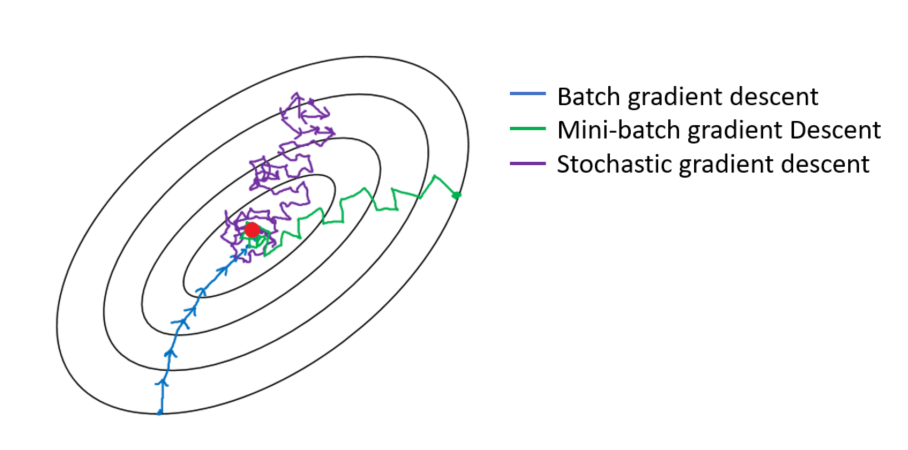
\includegraphics[width=0.6\textwidth]{images/img0.png}
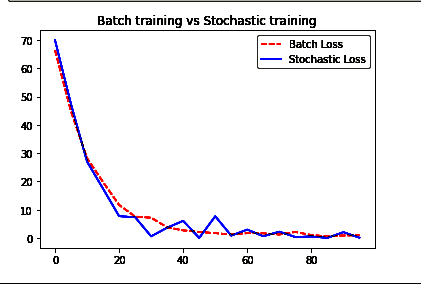
\includegraphics[width=0.4\textwidth]{images/img1.png}
\caption{(batch) Gradient Descent and Stochastic Gradient Descent}
\end{figure}
\subsection{Calculate the gradient of a function}
MATRIIX CALCULUS, EXAMPLES ECC\\ GRADIENT OF LP NORM AND OF REGRESSION LOSS (PG18 SECOND PDF)
\subsection{Convex functions and local minima}
check if the function is convex or not using the Hessian matrix... N<d: not enough data to estimate the parameters, X not full rank = not invertible\\
\subsection{Step size and learning rate choice}

\section{Measuring model performance}
in simple linear regression: r2, adj r2. generalize it to other models (logistic regression...).\\
Model optimism for model selection\\
Cross validation and choosing K (k-fold cross validation, leave one out cross validation ecc).\\
Precision and recall. tpr and fpr ecc... f1 score, balanced accuracy, Fowlkes-Mallow, Matthews Correlation, Jaccard Index, ROC curve, auc.\\
Pair-counting measures, rand index, mutual information

\section{Unsupervised learning}
blocco 3 mi pare

\section{Supervised learning}
blocco 4/5 mi pare

\end{document}